\chapter{\textsc{Compensation par retour de sortie dynamique - observateur fonctionnel}}
\addcontentsline{toc}{chapter}{\textsc{Compensation par retour de sortie dynamique - observateur fonctionnel}}
\chaptermark{\textsc{Compensation par retour de sortie dynamique - observateur fonctionnel}}
\section{\textsc{Observateur identité}}
\par Dans cette partie on veut construire un observateur identité à partir de l'entrée $v_m(t)$ et de la tension de sortie $v_s(t)=K_s\theta_s(t)$, mais également que l'observateur soit 2 fois, 4 fois puis 8 fois plus rapide que la dynamique de la boucle fermée.
\par On veut donc obtenir un système de cette forme :\\
~~\\
$\widehat{x}(t) = Mz(t) + Dy(t)$\\
$\dot{z}(t) = Fz(t)Gy(t) + Hu(t))$
\par Avec : H = B ; M = $I_{2}$ et D = 0.
\par On pose : $$F = \begin{bmatrix}f_{11} && f_{12} \\ f_{21} && f_{22} \end{bmatrix}~~~~et~~~~G = \begin{bmatrix}g_1 \\ g_2 \end{bmatrix}$$
\par Cela nous donne : 
$$F =  \begin{bmatrix}f_{11} && f_{12} \\ f_{21} && f_{22} \end{bmatrix} = \begin{bmatrix}0 && 10.5820 \\0 && -3.33 \end{bmatrix} - \begin{bmatrix}g_1 \\ g_2 \end{bmatrix}*\begin{bmatrix}1 && 0 \end{bmatrix}$$
\par A l'aide de Mathlab et la fonction "acker", nous avons calculé la matrice G et F :\\
~~\\
$P=[-2.4+5.5*i -2.4-5.5*i]\\
~~\\
G=acker(A’,C’,P)’\\
G1=acker(A’,C’,2*P)’\\
G2=acker(A’,C’,4*P)’\\
G3=acker(A’,C’,8*P)’\\
~~\\
F=A-G*C\\
F1=A-G1*C\\
F2=A-G2*C\\
F3=A-G3*C$


\paragraph{} D'où : $ F = \begin{bmatrix} -1.4667 && 10.5820 \\ -2.9409 && -3.3333 \end{bmatrix} $ et $ G = \begin{bmatrix}1.4667 \\ 2.9409\end{bmatrix} $\\
\par Par la suite, nous avons modélisé ce système à l'aide de Simulink notre schéma bloc, qui se présente de cette façon :
\begin{figure}[h!]
\centering
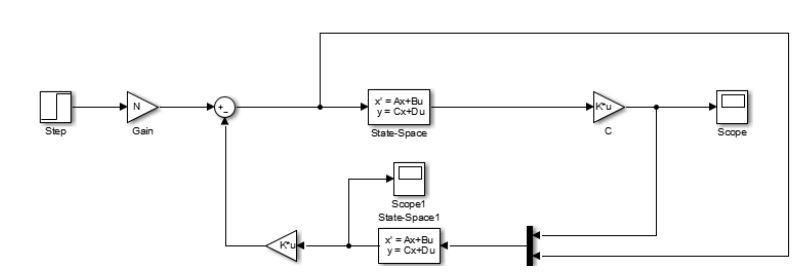
\includegraphics[scale = 0.7]{SIM1.JPG}\\[0.7 cm] 
\caption{Schéma bloc de l'observateur identité}
\end{figure}
\par La simulation donne donc :
\begin{figure}[h!]
\centering
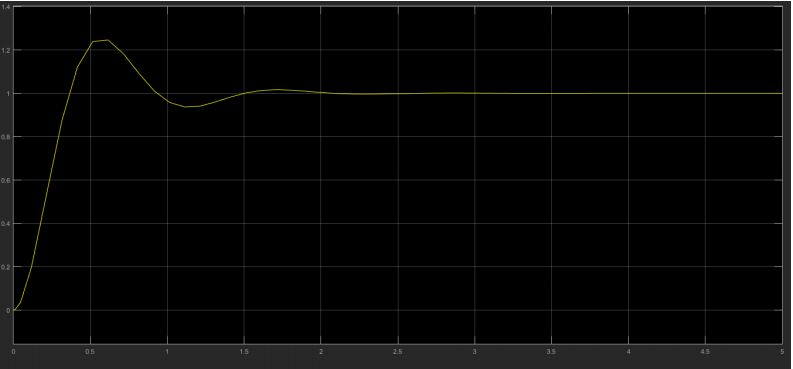
\includegraphics[scale = 0.7]{T1.JPG}\\[0.7 cm] 
\caption{Simulation observateur identité}
\end{figure}
\par On peut observer que le signal converge bien vers 1, qui est la consigne.
\par Ici nous avons calculé les gain de l'observateur de manière à modifier ses valeur propres pour que l'observateur soit d'abors 2 fois, puis 4 fois et enfin 8 fois plus rapide que la dynamique de la boucle fermée.
\par Pour cela nous avons multiplié par le nombre de fois qu'on veut les valeurs propres. Nous obtenon donc ceci :
$$F1 = \begin{bmatrix}-6.2667 && 10.5820 \\ -11.6378 && -3.3333\end{bmatrix}~~~~et~~~~G1 = \begin{bmatrix}6.2667 \\ 11.6378\end{bmatrix}$$
$$F2 = \begin{bmatrix}-15.8667 && 10.5820 \\ -49.4491 && -3.3333\end{bmatrix}~~~~et~~~~G2 = \begin{bmatrix}15.8667 \\ 49.4491\end{bmatrix}$$
$$F3 = \begin{bmatrix}-35.0667 && 10.5820 \\ -206.7425 && -3.3333\end{bmatrix}~~~~et~~~~G3 = \begin{bmatrix}35.0667 \\ 206.7425\end{bmatrix}$$
\par Nous avons ensuite modélisé trois observateur pour nos trois rapidité par des schéma bloc sur Simulink, comme montré ci-dessous :
\begin{figure}[h!]
\centering
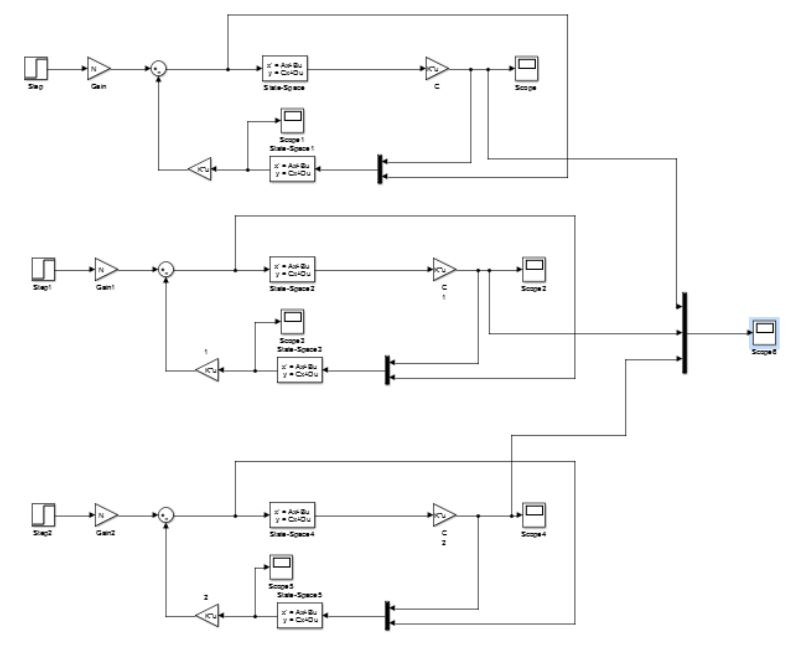
\includegraphics[scale = 0.7]{3OBS.JPG}\\[0.7 cm] 
\caption{Schéma bloc de trois observateurs}
\end{figure}
\pagebreak
\par Les tracés aux conditions initiales $v_s(0)=\pi/2~et~\dot{v_s}(0)=0$ nous donne évidemment trois courbes, qui sont de cette forme :
\begin{figure}[h!]
\centering
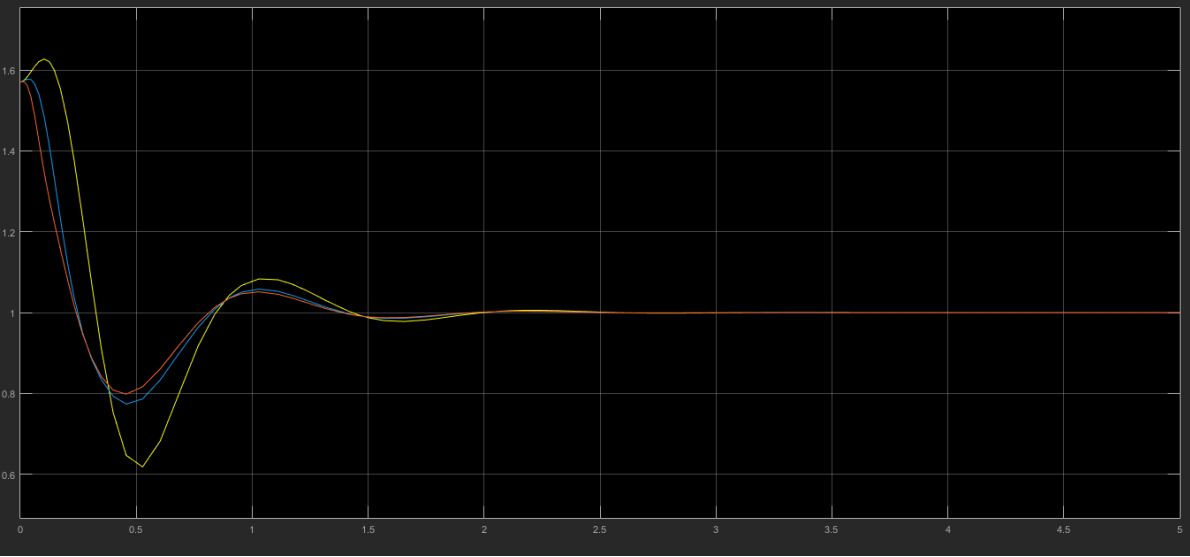
\includegraphics[scale = 0.45]{T_3OBS.JPG}\\[0.7 cm] 
\caption{Sortie des trois observateurs}
\end{figure}
\par On peut conclure que plus on augmente la valeur des valeurs propres et plus le système sera rapide d'où une convergence plus rapide des la sortie. De plus on observe une minime diminution du dépassement lorsque les valeurs propres augmentent.

\section{\textsc{Observateur minimal identité}}
\par Dans cette partie on veut construire un observateur minimal identité à partir de l'entrée $v_m(t)$ et de la tension de sortie $v_s(t)=K_s\theta_s(t)$, mais également que l'observateur sois 4 fois plus rapide que la dynamique de la boucle fermée.
\par On a notre matrice A, que l'on peut écrire de cette façon :
    $$A = \begin{bmatrix}0 && 10.5820 \\0 && -3.33 \end{bmatrix}$$
\par $A_{11}=0~; A_{12}=10.5820~; A_{21}=0~; A_{22}=3.33$
\par Et $B_1 = 0~~et~~B_2 = 3.5$
\par Dans cette partie notre nouveau système s'écrit de cette manière :\\
~~\\
$\dot{s}(t) = F_1s(t) + G_{tild}y(t)+H_{tild}u(t)$\\
$\widehat{z}(t) = s(t) + G_1y(t))$
\par On sait que :
$$G_{tild} = F_1G_1 - G_1A_{11} + A_{21}$$
$$H_{tild} = B_2G - GB_1$$
$$F_1=A_{22} - G_1A_{12}$$
\par En utilisant le code "acker" on peut calculer la valeur de G1, qui donne :
$G1=acker(A22’,A12’,4*(P))’$
\par Avec P=-2.4, cela nous donne :
$$G = 0.8190$$
D'où :
$$F = -9.6$$
Avec ces valeurs on peut calculer $G_{tild}$ et $H_{tild}$:
$$G_{tild} = -9.8280~~et~~H_{tild} = 3.5$$
\par Nous avons ensuite modélisé notre système sur Simulink par des schémas blocs :
\begin{figure}[h!]
\centering
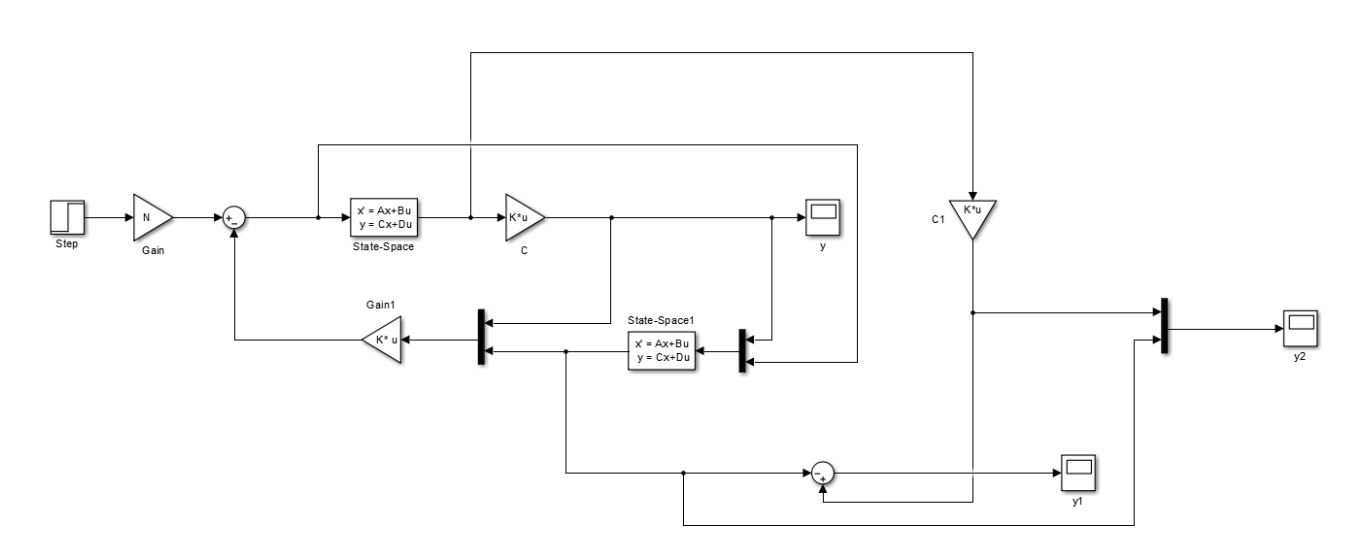
\includegraphics[scale = 0.35]{OBS_MINI.JPG}\\[0.7 cm] 
\caption{Schéma bloc de l'observateur minmal identité}
\end{figure}
\par La simulation avec des conditions initiales tel que, $v_s(0)=\pi/2~et~\dot{v_s}(0)=0$, nous obtenons en sortie de cet observateur minimal identité ceci :
\begin{figure}[h!]
\centering
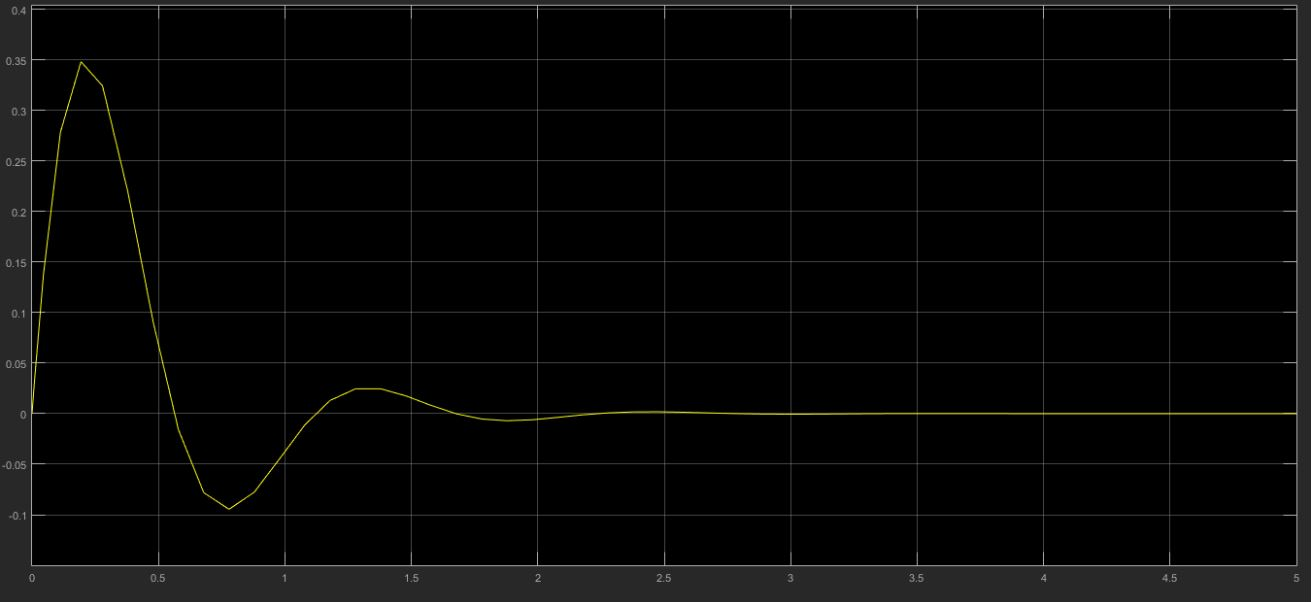
\includegraphics[scale = 0.35]{FFF1.JPG}\\[0.7 cm] 
\caption{Sortie du système avec observateur minmial identité}
\end{figure}
\par On peut conclure que le dépassement à énormément diminué comparé à l'observateur identité.


%(2)%%%%%%%%%%%%%%%%%%%%%%%%%%%%%%%%%%%%%%%%%%%%%%%%%%%%%%%%%%%%%%%%%%%%%%%%%%%%%%%%%%%%%%%%

\chapter{\textsc{Compensation par retour de sortie dynamique - observateur fonctionnel}}
\chaptermark{\textsc{Compensation par retour de sortie dynamique - observateur fonctionnel}}
\parindent=1cm 
Dans cette partie nous allons procéder à la reconstruction via un observateur fonctionnel permettant de reconstituer la valeur du retour d'état. C'est à dire un observateur qui converge vers $Kx(t)$, mais également  calculer les gains de l’observateur de manière à modifier ses valeurs propres pour que l’observateur soit 8 fois plus rapide que la dynamique de la boucle fermée. On veut donc $P_{min}=8*(-2.4)$
\par On a notre matrice A, que l'on peut écrire de cette façon :
    $$A = \begin{bmatrix}0 && 10.5820 \\0 && -3.33 \end{bmatrix}$$
\par $A_{11}=0~; A_{12}=105820~; A_{21}=0~; A_{22}=3.33$
\par Par la suite on veut résoudre ces équation : $$F_{fc}=A_{22}+T_1A_{12}$$ 
$$G_{fc} = A_{21} + T_1 A_{11} - F_{fc} T_1$$
$$ N_{fc} = k_1 - k_2T_1$$
$$H_{fc} = T  B$$
$$D'où~~~~M = k_2~~~~et~~~~T = [T_1~~1]$$
\par Il nous faut donc chercher la valeur de $T_1$. A l'aide de mathlab on utilise la fonction "acker", ce qui donne : $$T_1 = acker (A_{22}’,-A_{12}’,P_{min} ) = -1.4994$$
\par On obtient donc : $$F_{fc} = -19.2$$
\par D'où : $$G_{fc} = -287885$$
\par Puis : $$N_{fc} = 1.6006$$
\par Et : $$H_{fc} = 3.5$$
\par On peut donc écrire notre nouveau système se présentant sous cette forme :
$$A_{fc} = F_{fc}~~;~~B_{fc} = [G_{fc}~~H_{fc}]~~;
~~C_{fc} = M~~;~~D_{fc} = [N_{fc}~~0]$$

\par Nous avons par la suite modélisé le schéma bloc du système sous Simulink de cette manière :
\begin{figure}[h!]
\centering
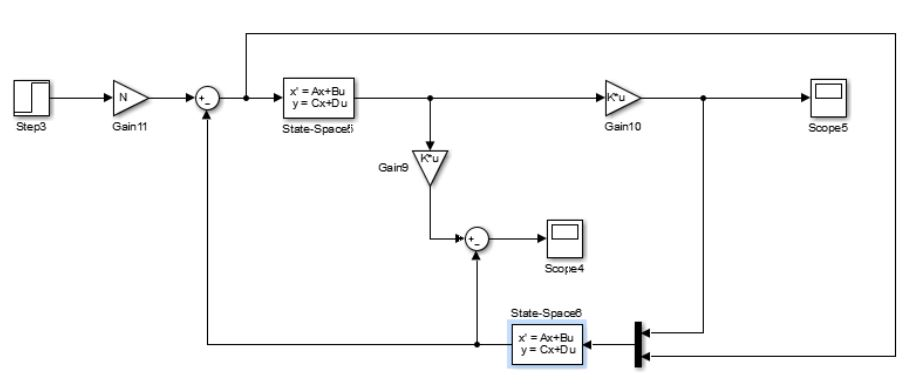
\includegraphics[scale = 0.5]{Capture.JPG}\\[0.7 cm] 
\caption{Schéma bloc observateur fonctionnel}
\end{figure}
\par La simulation avec des conditions initiales nulles ($v_s(0)=0~et~\dot{v_s}(0)=0$) nous donne un tracé comme montré ci-dessous :
\begin{figure}[h!]
\centering
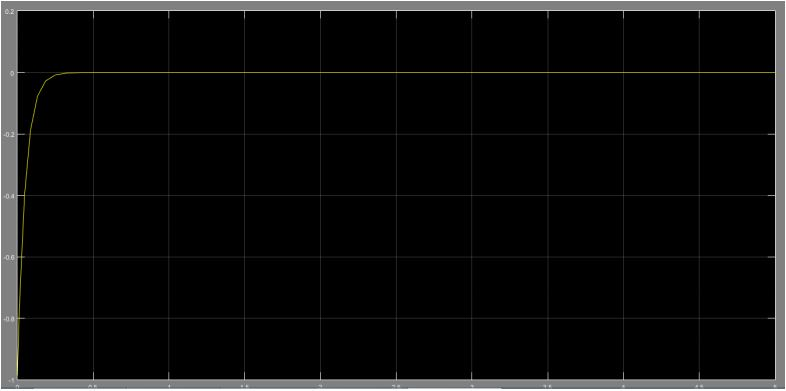
\includegraphics[scale = 0.7]{S1.JPG}\\[0.7 cm] 
\caption{Sortie du système avec observateur fonctionnel et conditions initiales nulles}
\end{figure}
\pagebreak
\par Maintenant avec des conditions initiales différentes ($v_s(0)=\pi/2~et~\dot{v_s}(0)=0$), on obtient un tracé comme montré ci-dessous :
\begin{figure}[h!]
\centering
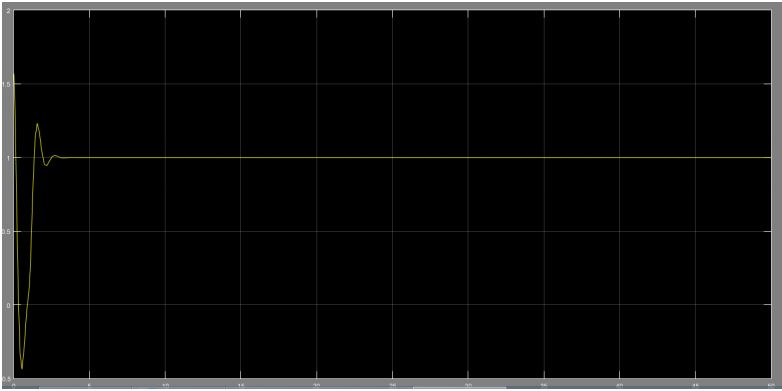
\includegraphics[scale = 0.7]{S2.JPG}\\[0.7 cm] 
\caption{Sortie du système avec observateur fonctionnel et conditions initiales différente}
\end{figure}
\par L'objectif a été atteint, car d'après le tracé on a une sortie qui est plus rapide avec le nouvel observateur fonctionnel.
